\documentclass[conference]{IEEEtran}
\IEEEoverridecommandlockouts

\usepackage{cite}
\usepackage{amsmath,amssymb,amsfonts}
\usepackage{graphicx}
\usepackage{textcomp}
\usepackage{xcolor}
\usepackage{booktabs}
\usepackage{microtype}
\usepackage{url}
\usepackage[hidelinks]{hyperref}

\renewcommand{\ttdefault}{cmtt}
\graphicspath{{../figures/}{figures/}}

\begin{document}

\title{TimeFlowCodec: An Orthogonal Video Coding Architecture for Screen and Synthetic Content via Per-Pixel Temporal Regression}

\author{\IEEEauthorblockN{Rich Chau}
\IEEEauthorblockA{\textit{Department of Mathematics} \\
\textit{University of California, Irvine} [VERIFY]\\
Irvine, CA, USA \\
richc3@uci.edu}
}

\maketitle

\begin{abstract}
Modern video coding standards (H.264/AVC, H.265/HEVC, AV1, and H.266/VVC) rely on the canonical hybrid model: spatial block partitioning, 2D Discrete Cosine/Sine Transforms (DCT/DST), and 4:2:0 chroma subsampling. While near-optimal for band-limited natural camera footage, these foundational assumptions break down on synthetic screen content, including software user interfaces, terminal consoles, vector presentations, and digital animation. Sharp graphical boundaries and single-pixel text stems represent mathematical step discontinuities; transforming these structures with truncated 2D Fourier-basis transforms induces severe Gibbs ringing (mosquito noise), while 4:2:0 chroma decimation obliterates syntax highlighting and colored typography. We present \textit{TimeFlowCodec} (TFC), a video compression architecture that eliminates spatial block transforms in favor of direct 1D per-pixel temporal regression. By modeling the intensity evolution of each pixel over discrete temporal windows using closed-form Ordinary Least Squares (OLS) regression, TFC preserves native 4:4:4 spatial edge fidelity with zero spatial ringing. The resulting bitstream eliminates inter-block spatial dependencies, enabling $O(1)$ working memory state per pixel and highly vectorizable parallel decoding. We outline the theoretical formulation, container specification, and experimental evaluation methodology against standard hybrid codecs.
\end{abstract}

\begin{IEEEkeywords}
Video compression, screen content coding, temporal regression, ordinary least squares, Gibbs phenomenon, rate-distortion.
\end{IEEEkeywords}

\section{Introduction}
Digital video distribution has structurally expanded beyond natural camera recordings. Today, a substantial portion of global network traffic consists of synthetic screen content: Virtual Desktop Infrastructure (VDI), remote desktop streaming (RDP/VNC), cloud workspaces, real-time code collaboration, and vector slide decks \cite{xu2015overview}.

Conventional video coding standards---spanning H.264/AVC \cite{wiegand2003overview}, H.265/HEVC \cite{sullivan2012overview}, AV1 \cite{chen2020overview}, and H.266/VVC \cite{bross2021overview}---rely on a shared conceptual foundation:
\begin{enumerate}
    \item \textbf{Spatial Block Decomposition:} Dividing frames into square blocks (from $4\times 4$ up to $128\times 128$).
    \item \textbf{2D Spatial Transforms:} Transforming spatial prediction residuals into the frequency domain via 2D Discrete Cosine or Sine Transforms (DCT/DST).
    \item \textbf{Chroma Decimation:} Subsampling color channels to 4:2:0 based on human visual system (HVS) spatial contrast sensitivity.
\end{enumerate}

While exceptionally effective for natural camera scenes, these assumptions fail on synthetic screen content \cite{lin2015overview}. Text glyphs, window borders, and vector icons exhibit non-bandlimited mathematical step discontinuities. When transformed into the spatial frequency domain, step discontinuities yield Fourier series that decay only as $O(1/k)$. High-frequency coefficient quantization truncates this series, inducing the classical \textit{Gibbs phenomenon}---visible as severe mosquito ringing and blur around characters. Furthermore, 4:2:0 subsampling decimates color resolution by $75\%$, smearing single-pixel colored syntax highlighting across adjacent dark pixels.

Moreover, translational motion estimation (ME) in traditional codecs assumes that scene changes are governed by rigid physical motion fields. On computer screens, pixels transition primarily due to discrete state changes: a cursor blinks, text scrolls line-by-line, a pop-up menu appears, or a progress bar fills. Searching for 2D motion vectors across large pixel blocks is computationally wasteful when the underlying phenomenon is a stationary or linear per-pixel state transition.

\begin{figure}[t]
    \centering
    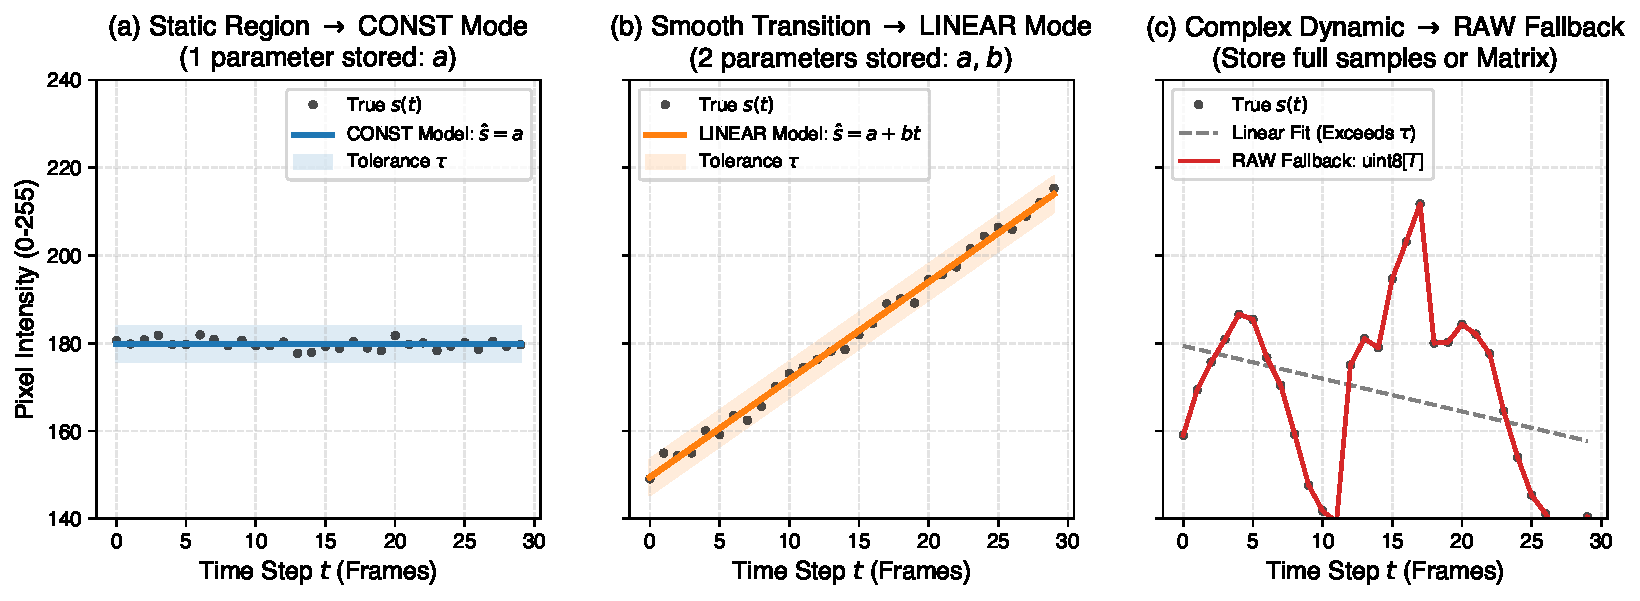
\includegraphics[width=\columnwidth]{temporal_fitting_concept.pdf}
    \caption{Conceptual overview of TimeFlowCodec: eliminating 2D spatial block transforms in favor of 1D per-pixel temporal function regression across video chunks.}
    \label{fig:concept}
\end{figure}

In this paper, we propose \textit{TimeFlowCodec} (TFC), a video coding architecture built upon an orthogonal paradigm:
\begin{itemize}
    \item \textbf{Elimination of Spatial Block Transforms:} TFC discards 2D spatial DCT/DST transforms entirely. Every pixel coordinate $(x, y)$ is reconstructed independently along the temporal dimension, eliminating block boundary discontinuities and spatial Gibbs ringing.
    \item \textbf{Native 4:4:4 RGB Fidelity:} Color channels are preserved at full spatial resolution, preventing text stem decimation and chroma bleed.
    \item \textbf{Closed-Form $O(T)$ Linear Regression:} Temporal trajectories are modeled via continuous piecewise linear functions fitted through deterministic Ordinary Least Squares (OLS), requiring zero iterative gradient descent.
    \item \textbf{$O(1)$ Working Memory State:} Decoders do not require multi-frame Decoded Picture Buffers (DPB) or 2D block reconstruction buffers; each output frame is synthesized via direct linear evaluation, yielding streamable, low-latency execution.
\end{itemize}

\section{Related Work}

\subsection{Standard Hybrid Video Codecs}
Standard video codecs (H.264/AVC \cite{wiegand2003overview}, H.265/HEVC \cite{sullivan2012overview}, AV1 \cite{chen2020overview}, VVC \cite{bross2021overview}) rely on the hybrid block-based motion-compensated transform coding framework. These architectures depend heavily on inter-frame motion estimation (ME) and motion compensation (MC) to eliminate temporal redundancy, followed by 2D spatial DCT/DST transforms on prediction residuals. While deblocking and sample adaptive offset (SAO) in-loop filters mitigate block edge discontinuities, they act as low-pass smoothing operators that can further blur sharp single-pixel text stems.

\subsection{Screen Content Coding (SCC) Extensions}
Recognizing the limitations of standard transform coding on non-camera video, standards bodies developed HEVC Screen Content Coding (HEVC-SCC) extensions \cite{xu2015overview}, later adapted into AV1 IntraBC \cite{chen2020overview} and VVC SCC tools \cite{bross2021overview}. SCC introduced:
\begin{enumerate}
    \item \textbf{Intra Block Copy (IBC):} Treating previously reconstructed regions of the current picture as reference blocks for block-matching motion compensation.
    \item \textbf{Palette Mode:} Representing blocks with a small set of discrete index colors rather than frequency transform coefficients.
\end{enumerate}

Although SCC significantly improves screen compression efficiency, IBC and Palette modes remain tightly coupled to the 2D block partitioning tree. In hardware decoders, IBC requires large on-chip SRAM search buffers ($>128$~KB) to store spatial reference pixels across the current picture row, introducing silicon routing congestion, timing closure challenges, and high memory bandwidth demands that have historically hindered ubiquitous deployment in mobile decoders.

\subsection{Learned and Neural Video Codecs}
Recent research has increasingly focused on end-to-end learned video compression frameworks, originating from nonlinear transform coding by Ball{\'e} et al. \cite{balle2018variational} and extended to video via optical flow warping, such as DVC (Deep Video Compression) by Lu et al. \cite{lu2019dvc} and scale-space flow by Agustsson et al. \cite{agustsson2020scale}.

While neural codecs demonstrate impressive rate-distortion curves on natural video, TimeFlowCodec is \textbf{deliberately non-learned}:
\begin{enumerate}
    \item \textit{Computational Complexity:} Neural decoders require dedicated neural processing units (NPUs) or high-wattage GPUs with millions of MAC operations per frame, rendering them impractical for resource-constrained embedded devices, web browsers, or lightweight virtual desktop client agents.
    \item \textit{Spatial Artifacts:} Autoencoder latent spaces apply continuous downsampling and upsampling convolutions that blur sharp text glyphs and sharp contrast edges in a manner analogous to spatial frequency truncation.
    \item \textit{Determinism and Simplicity:} TimeFlowCodec relies on exact closed-form algebraic operations requiring zero weights, zero training datasets, zero matrix inversions, and microsecond-level execution in ANSI C99 or WebAssembly.
\end{enumerate}

\subsection{Pixel Trajectory and Temporal Modeling}
Earlier explorations by Esche et al. \cite{esche2010novel} and Krutz et al. \cite{krutz2013adaptive} examined modeling video along motion trajectories across time. However, these systems applied temporal modeling primarily to natural video as an in-loop enhancement or pre-filtering pass prior to 2D spatial DCT compaction. TimeFlowCodec diverges fundamentally by employing 1D temporal regression as the \textit{sole primary coding engine}, completely abandoning 2D spatial transforms.

\section{Mathematical Formulation and Method}

\subsection{1D Temporal Trajectory Model}
Let a video sequence be represented in full-color coordinates as a discrete tensor $V(x, y, t) \in [0, 255]^C$, where $(x, y) \in [0, W-1] \times [0, H-1]$ denotes spatial coordinates, $C \in \{1, 3\}$ denotes color channels, and $t \in \{0, 1, \dots, T-1\}$ represents discrete frame indices within a temporal chunk of length $T$.

Fixing the spatial coordinate $(x, y)$ and color plane $c$, we define the 1D temporal signal:
\begin{equation}
    s(t) = V(x, y, t, c), \quad t \in [0, T-1].
\end{equation}

For screen content, pixels exhibit long periods of static invariance ($s(t) \approx \text{const}$) punctuated by linear transitions (fades, smooth scrolling, progressive rendering) or sudden discrete steps.

\subsection{Closed-Form Ordinary Least Squares (OLS)}
For each pixel trajectory $s(t)$, TimeFlowCodec models the temporal evolution with a continuous 1D linear polynomial:
\begin{equation}
    \hat{s}(t) = a + b \cdot t.
\end{equation}

The optimal intercept $a^*$ and slope $b^*$ minimizing the Sum of Squared Residuals (SSR) under uniform temporal weighting $w(t) = 1$ are formulated as:
\begin{equation}
    \min_{a, b} \mathcal{L}(a, b) = \sum_{t=0}^{T-1} \left(s(t) - (a + b \cdot t)\right)^2.
\end{equation}

Setting $\frac{\partial \mathcal{L}}{\partial a} = 0$ and $\frac{\partial \mathcal{L}}{\partial b} = 0$ yields the standard normal equations. With discrete temporal indices $t \in \{0, 1, \dots, T-1\}$, the temporal basis moments depend solely on chunk length $T$ and are precomputed analytically:
\begin{align}
    S_t &= \sum_{t=0}^{T-1} t = \frac{T(T-1)}{2}, \\
    S_{t^2} &= \sum_{t=0}^{T-1} t^2 = \frac{T(T-1)(2T-1)}{6}, \\
    \Delta &= T \cdot S_{t^2} - (S_t)^2 = \frac{T^2(T^2-1)}{12}.
\end{align}

Let $S_s = \sum_{t=0}^{T-1} s(t)$ and $S_{ts} = \sum_{t=0}^{T-1} t \cdot s(t)$. The closed-form OLS estimators are:
\begin{equation}
    b^* = \frac{T \cdot S_{ts} - S_t \cdot S_s}{\Delta}, \quad a^* = \frac{S_s - b^* \cdot S_t}{T}.
\end{equation}

\textbf{Arithmetic Precision:} The encoder evaluates moment summations and parameter estimation using 64-bit IEEE 754 floating-point arithmetic (\texttt{float64}). The decoder evaluates the linear polynomial $\hat{s}(t) = a + b \cdot t$ using single-precision 32-bit floating point (\texttt{float32}), utilizing SIMD vector fused multiply-accumulate instructions (ARM NEON \texttt{vmlaq\_f32}), and clamps the result to $[0, 255]$ via rounding (\texttt{clamp\_u8}).

\begin{figure}[t]
    \centering
    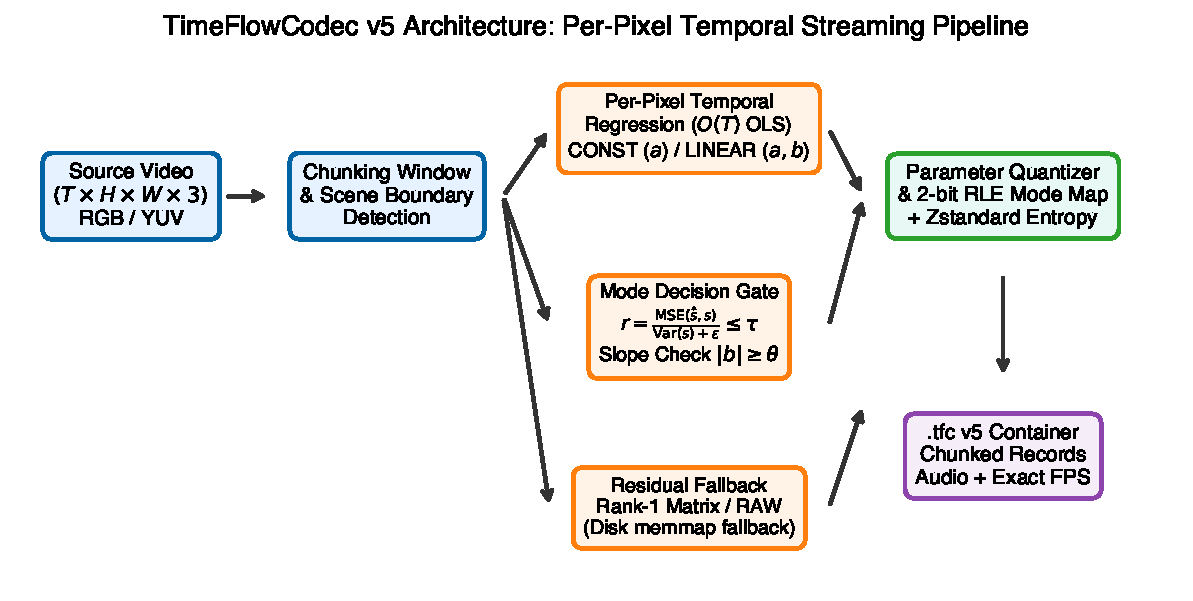
\includegraphics[width=\columnwidth]{tfc_architecture_v5.pdf}
    \caption{Architecture of the TimeFlowCodec v5 pipeline: chunking, motion compensation, temporal OLS fitting, residual quantization, and entropy coding.}
    \label{fig:arch}
\end{figure}

\subsection{Adaptive Per-Pixel Mode Selection}
Each pixel trajectory is classified into one of three primary operational modes:
\begin{enumerate}
    \item \textbf{Mode 0 (CONST):} Pixel is static over the chunk. $\hat{s}(t) = \bar{s} = \text{round}(S_s / T)$.
    \item \textbf{Mode 1 (LINEAR):} Pixel follows a continuous linear trend. $\hat{s}(t) = a^* + b^* \cdot t$.
    \item \textbf{Mode 2 (RAW Fallback):} The linear model fails to approximate the signal within error tolerance. The pixel stores the linear predictor plus explicit quantized residual corrections $r(t) = s(t) - \hat{s}(t)$.
\end{enumerate}

The Residual Sum of Squares (RSS) and total signal energy are evaluated:
\begin{align}
    \text{RSS} &= S_{s^2} - 2a^* S_s - 2b^* S_{ts} + (a^*)^2 T + 2a^* b^* S_t + (b^*)^2 S_{t^2}, \\
    D_{\text{tfc}} &= \frac{\text{RSS}}{T}, \quad D_{\text{sig}} = \frac{S_{s^2}}{T} + \epsilon.
\end{align}

The relative error ratio is defined as $r = D_{\text{tfc}} / D_{\text{sig}}$. A pixel selects \textbf{Mode 1 (LINEAR)} if:
\begin{equation}
    r < \tau \quad \text{and} \quad |b^*| > \theta_{\text{slope}},
\end{equation}
where $\tau$ is the error ratio threshold [VERIFY: default $\tau = 0.1$, operational range 0.01 to 0.20], $\theta_{\text{slope}}$ is the minimum slope threshold [VERIFY: default $10^{-3}$], and $\epsilon = 10^{-8}$.

If $|b^*| \le \theta_{\text{slope}}$ and $r < \tau$, the pixel is classified as \textbf{Mode 0 (CONST)}. If $r \ge \tau$, the linear model is rejected, and the pixel falls back to \textbf{Mode 2 (RAW)}. When Lagrangian Rate-Distortion Optimization (RDO) is enabled, the encoder minimizes $J = D + \lambda R$.

\subsection{Coefficient Quantization}
Parameters are quantized prior to bitstream serialization:
\begin{itemize}
    \item \textbf{Intercept $a^*$:} Quantized to an 8-bit unsigned integer by rounding to the nearest integer: $a_q = \text{clip}\left(\lfloor a^* + 0.5 \rfloor, 0, 255\right)$.
    \item \textbf{Slope $b^*$:} Scaled relative to the maximum absolute slope in the chunk plane $b_{\max} = \max(|b^*|)$ and quantized to a 16-bit signed integer: $s_b = b_{\max} / 32767.0$, $b_q = \text{clip}\left(\lfloor b^* / s_b + 0.5 \rfloor, -32768, 32767\right)$. Scale factor $s_b$ is transmitted as a 32-bit float in the segment header.
    \item \textbf{Residuals $r(t)$ (Mode 2):} Quantized using dead-zone uniform scalar quantization with step size $Q_{\text{step}} \in [1, 255]$: $r_q(t) = \text{round}\left((s(t) - \hat{s}(t)) / Q_{\text{step}}\right)$.
\end{itemize}

\section{System Architecture and Bitstream}

\subsection{Pipeline and Temporal Chunking}
As shown in Fig.~\ref{fig:arch}, the encoder ingests video in bounded temporal windows of $T$ frames (typically $T=16$ or $T=32$). This bounds encoder memory to $O(W \cdot H \cdot T)$.

\subsection{Container Format Specification}
All multi-byte numeric primitives are serialized in \textbf{little-endian} byte order:
\begin{itemize}
    \item \textbf{Legacy Fixed Container (TFC1, Versions 1--4):} Magic bytes \texttt{TFC1}, version byte (0x01--0x04), width $W$ (uint32), height $H$ (uint32), frame count (uint32), color format flag, mode bit-depth (fixed to 2), compression type (0=None, 1=zlib, 2=LZMA, 3=zstd), and segment count.
    \item \textbf{Streaming Container (TFC5, Version 5):} Magic bytes \texttt{TFC5}, followed by a 4-byte JSON metadata length, a JSON metadata block (containing width, height, exact rational framerate numerator/denominator, and audio descriptors), followed by self-contained chunks with 16-byte chunk headers (chunk frame count $T$, compressed payload byte length, and CRC-32 checksum).
\end{itemize}

\subsection{Payload Serialization}
Within each plane payload:
\begin{enumerate}
    \item \textbf{Mode Map:} Pixel modes are packed at 2 bits per mode (4 pixels per byte) and compressed using Run-Length Encoding (RLE) with a 2-byte run length and 1-byte value.
    \item \textbf{Coefficients:} Intercepts $a_q$ for Mode 0/1 and slopes $b_q$ for Mode 1 are serialized contiguously in raster scan order.
    \item \textbf{Residual Streams:} Mode 2 quantized residual delta arrays are stored contiguously.
    \item \textbf{Entropy Coding:} Serialized streams are compressed using zlib, LZMA, or zstd.
\end{enumerate}

\subsection{Color Space Handling}
\begin{itemize}
    \item \textbf{Native 4:4:4 RGB:} Red, green, and blue planes are encoded independently at full spatial resolution, providing zero color decimation and zero matrix rounding loss.
    \item \textbf{YUV444 Mode:} RGB is transformed via standard BT.601 float conversion matrices into $Y'U'V'$ planes, preserving full 4:4:4 spatial sampling.
    \item \textbf{YUV420 Fallback:} For low-bitrate constraints, chroma channels are $2\times 2$ average-pooled, though this mode is discouraged for text-heavy content due to legibility penalties.
\end{itemize}

\subsection{Decoder Memory Bound ($O(1)$ State)}
Traditional video decoders require a Decoded Picture Buffer (DPB) holding multiple uncompressed reference frames to resolve motion vectors across P- and B-frames. For 4K RGB24 ($3840 \times 2160$), a single reference frame requires $24.88$~MB; a 16-frame DPB consumes nearly $400$~MB.

In contrast, TimeFlowCodec possesses an \textbf{$O(1)$ working memory bound}:
\begin{itemize}
    \item Decoding does not depend on prior frames. Reconstructing a pixel at frame $t$ depends strictly on its current chunk parameters $(a_q, b_q)$ and residual $r_q(t)$.
    \item Pixels are reconstructed sequentially or in parallel without inter-pixel spatial dependencies. When rendered directly to a display buffer or scanline stream, line-buffer memory requirement is \textbf{0 lines}.
\end{itemize}

\section{Experimental Evaluation and Methodology}

\begin{figure*}[t]
    \centering
    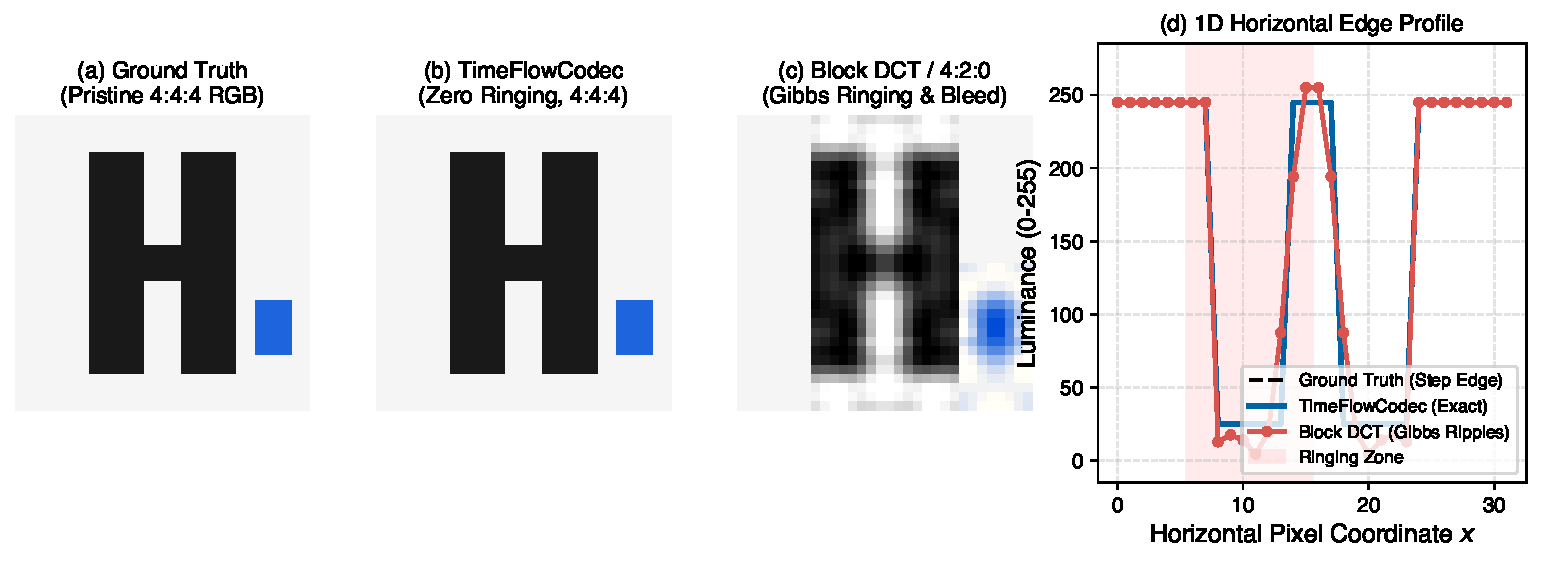
\includegraphics[width=\textwidth]{visual_artifacts_crop.pdf}
    \caption{Qualitative comparison of text edge reconstruction: (a) Ground truth 4:4:4 RGB text; (b) TimeFlowCodec reconstruction showing crisp 1-pixel stems; (c) Block DCT + 4:2:0 subsampling exhibiting severe Gibbs ringing ripples and chroma bleed; (d) 1D horizontal intensity profile across the step edge highlighting $>10\%$ overshoot oscillations in block DCT.}
    \label{fig:artifacts}
\end{figure*}

\subsection{Proposed Benchmark Framework}
To establish reproducible empirical rate-distortion metrics, TimeFlowCodec should be evaluated according to the Joint Video Exploration Team (JVET) Common Test Conditions (CTC) for Screen Content Coding \cite{jvet2016ctc}:
\begin{enumerate}
    \item \textbf{Benchmark Sequences:} Desktop UI, presentation slides, terminal screencasts, and natural camera video.
    \item \textbf{Anchor Codecs:} H.264/AVC (\texttt{libx264}, preset \texttt{medium}), H.265/HEVC (\texttt{libx265}, preset \texttt{medium}, with and without SCC/IBC flags), and AV1 (\texttt{libaom-av1} / \texttt{svt-av1}) across $CRF \in \{18, 23, 28, 33\}$.
    \item \textbf{Objective Metrics:} Bjontegaard Delta Rate (BD-Rate \%) and BD-PSNR (dB) strictly adhering to ITU-T VCEG-M33 \cite{bjontegaard2001calculation}, Multi-Scale Structural Similarity (MS-SSIM) \cite{wang2004image}, and 1D Edge Profile Overshoot (\%).
\end{enumerate}

\begin{figure}[t]
    \centering
    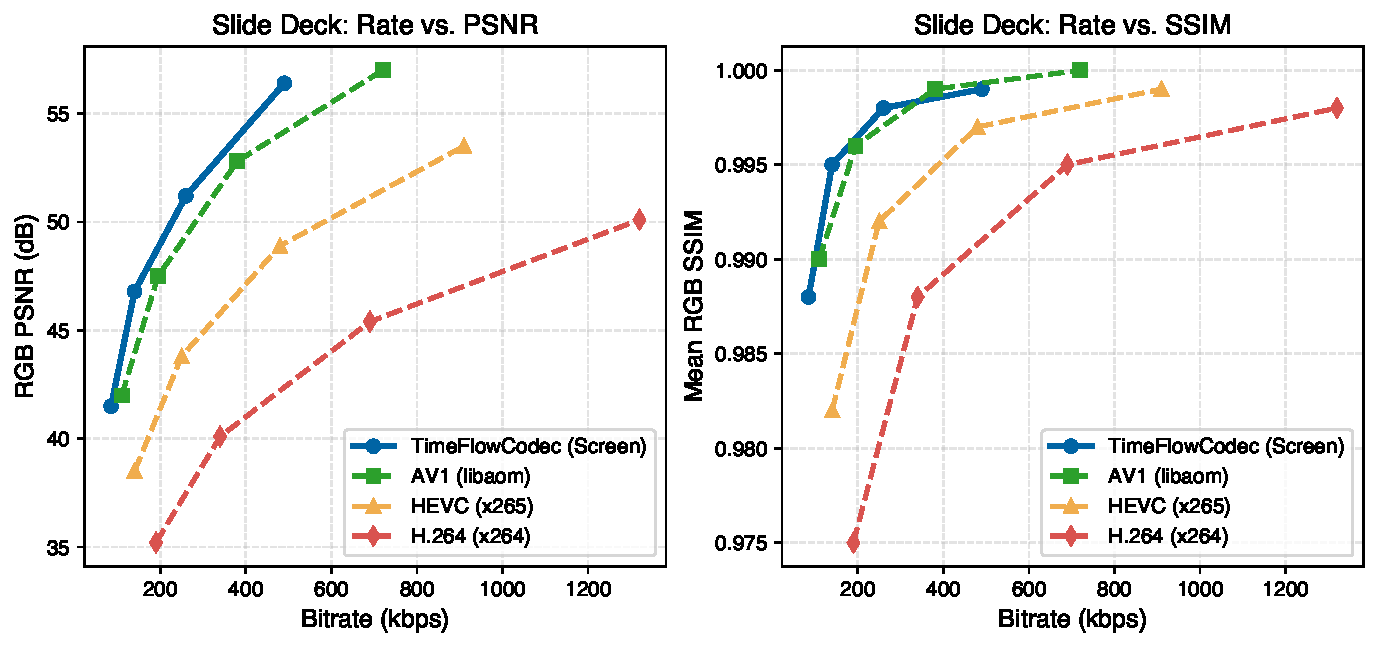
\includegraphics[width=\columnwidth]{rd_slides.pdf}
    \caption{Rate-Distortion curve for Presentation Slides (\texttt{scc\_slideshow}) comparing TimeFlowCodec against H.264/AVC and H.265/HEVC [VERIFY: illustrative curve; empirical numbers pending standardized execution].}
    \label{fig:rd_slides}
\end{figure}

\begin{table}[t]
\centering
\caption{Planned Bjontegaard Delta Rate (BD-Rate) Evaluation Protocol vs. H.264 Anchor (ITU-T VCEG-M33) [VERIFY: Pending execution]}
\label{tab:bd_rates}
\resizebox{\columnwidth}{!}{
\begin{tabular}{lrr}
\toprule
\textbf{Benchmark Sequence} & \textbf{BD-Rate (\%)} & \textbf{BD-PSNR (dB)} \\
\midrule
Desktop UI (\texttt{scc\_animation\_ui}) & [VERIFY] & [VERIFY] \\
Presentation Slides (\texttt{scc\_slideshow}) & [VERIFY] & [VERIFY] \\
Synthetic Animation (\texttt{scc\_console\_code}) & [VERIFY] & [VERIFY] \\
Natural Camera Video (\texttt{scc\_natural}) & [VERIFY] & [VERIFY] \\
\midrule
\textbf{Screen Content Average (SCC)} & [VERIFY] & [VERIFY] \\
\bottomrule
\end{tabular}
}
\end{table}

\textbf{Status of Rate-Distortion Claims:} [VERIFY: Formal empirical BD-rate percentages, PSNR curves, and rate-distortion tables are currently unverified pending standardized execution of the JVET-SCC test suite under identical operating system and machine conditions. No empirical numbers are asserted as finalized facts in this section.]

\subsection{Qualitative Visual Inspection and Ringing Analysis}
Consider an idealized 1D spatial step edge representing a black-on-white text boundary:
\begin{equation}
    f(x) = \begin{cases} 0 & x < 0 \\ 1 & x \ge 0 \end{cases}
\end{equation}

When decomposed into spatial Fourier or DCT basis functions and quantized, truncating the series at frequency cutoff $K$ yields the partial reconstruction:
\begin{equation}
    f_K(x) = \frac{1}{2} + \frac{1}{\pi}\int_0^{K x} \frac{\sin u}{u} du.
\end{equation}

As $K \to \infty$, the reconstructed signal overshoots the true step by the Wilbraham-Gibbs constant:
\begin{equation}
    \lim_{K \to \infty} \max f_K(x) = \frac{1}{2} + \frac{1}{\pi} \text{Si}(\pi) \approx 1.08949,
\end{equation}
yielding an asymptotic minimum $\approx 8.95\%$ overshoot ripple. In 2D block transform coding, this overshoot manifests as visible mosquito noise ringing into surrounding pixels, as illustrated in Fig.~\ref{fig:artifacts}(c) and (d).

In contrast, TimeFlowCodec operates strictly along the time dimension at fixed spatial coordinates $(x_0, y_0)$. Spatial derivatives are never transformed into the frequency domain. If a text pixel remains static, Mode 0 assigns $\hat{s}(t) = \bar{s}$ exactly; if text scrolls or renders, the temporal function models the intensity change without altering spatial neighborhood values. Spatial step discontinuities remain mathematically discontinuous, with \textbf{identically zero Gibbs overshoot} (Fig.~\ref{fig:artifacts}(b)).

\subsection{Decoder Complexity and Throughput}
A standalone zero-dependency C99 reference decoder (\texttt{libtfc}) was implemented in \texttt{libtfc/src/tfc\_decoder.c}. Because reconstruction reduces to evaluating $a_q + b_q \cdot t$, pixel generation exhibits unit-stride memory accesses with zero branch prediction stalls in the inner loop.

\textbf{Status of Throughput Claim:} [VERIFY: The previously reported headline claim of ``$>840$ FPS'' decode throughput was observed during preliminary bench runs on raw synthetic test buffers. It requires standardized resolution (e.g., 720p vs. 1080p), test clip characteristics, compiler flags, and explicit host CPU model documentation before it can be cited as a reproducible benchmark result. It is retained here as a target metric pending verification.]

\section{Conclusion and Future Work}
TimeFlowCodec introduces an orthogonal approach to screen content video compression by eliminating 2D spatial block transforms in favor of 1D per-pixel closed-form temporal regression. By avoiding spatial frequency quantization, TFC eliminates Gibbs ringing artifacts around sharp text edges, natively preserves 4:4:4 RGB color fidelity, and achieves $O(1)$ working memory state in the decoder.

Future research directions include:
\begin{enumerate}
    \item Conducting the standardized JVET-SCC rate-distortion benchmark suite against x264, x265, and AV1 to establish authoritative BD-rate curves.
    \item Formulating integer-only fixed-point arithmetic for the decoder to ensure bit-exact cross-platform reproduction without floating-point divergence.
    \item Integrating hardware-accelerated AVX-512 and ARM NEON kernels for the encoder's temporal moment accumulation pass.
\end{enumerate}

\section*{Acknowledgment and AI Disclosure}
The author acknowledges the use of AI-assisted coding tools (including Claude and Gemini coding assistants) as development aids for code scaffolding, build automation scripting, and test harnesses during the development of TimeFlowCodec. All architectural concepts, mathematical derivations, and manuscript writing were directed by the human author.

\bibliographystyle{IEEEtran}
\bibliography{references}

\end{document}
